\documentclass[12pt,a4paper]{article}
\usepackage{hyperref} % Use the Charter font for the document text
%\usepackage[UTF8]{ctex}
\usepackage{fullpage}
\usepackage{amsfonts,amssymb,amsmath}
\usepackage{mathtools}
\usepackage{tikz-cd}
\usepackage{tikz}

\usepackage{alltt}
\usepackage{amsfonts}
\usepackage{amsmath}
\usepackage{amssymb}
\usepackage{amsthm}
\usepackage{booktabs}
\usepackage{caption}
\usepackage{enumitem}
\usepackage{fancyhdr}
\usepackage{graphicx}
\usepackage{mathdots}
\usepackage{mathtools}
\usepackage{microtype}
\usepackage{multirow}
\usepackage{pdflscape}
\usepackage{pgfplots}
\usepackage{siunitx}
\usepackage{slashed}
\usepackage{tabularx}
\usepackage{tikz}
\usepackage{tkz-euclide}
\usepackage[normalem]{ulem}
\usepackage[all]{xy}
\usepackage{imakeidx}

\newcommand{\bA}{\ensuremath{\mathbb{A}}}
\newcommand{\bB}{\ensuremath{\mathbb{B}}}
\newcommand{\bC}{\ensuremath{\mathbb{C}}}
\newcommand{\bD}{\ensuremath{\mathbb{D}}}
\newcommand{\bE}{\ensuremath{\mathbb{E}}}
\newcommand{\bF}{\ensuremath{\mathbb{F}}}
\newcommand{\bG}{\ensuremath{\mathbb{G}}}
\newcommand{\bH}{\ensuremath{\mathbb{H}}}
\newcommand{\bI}{\ensuremath{\mathbb{I}}}
\newcommand{\bJ}{\ensuremath{\mathbb{J}}}
\newcommand{\bK}{\ensuremath{\mathbb{K}}}
\newcommand{\bL}{\ensuremath{\mathbb{L}}}
\newcommand{\bM}{\ensuremath{\mathbb{M}}}
\newcommand{\bN}{\ensuremath{\mathbb{N}}}
\newcommand{\bO}{\ensuremath{\mathbb{O}}}
\newcommand{\bP}{\ensuremath{\mathbb{P}}}
\newcommand{\bQ}{\ensuremath{\mathbb{Q}}}
\newcommand{\bR}{\ensuremath{\mathbb{R}}}
\newcommand{\bS}{\ensuremath{\mathbb{S}}}
\newcommand{\bT}{\ensuremath{\mathbb{T}}}
\newcommand{\bU}{\ensuremath{\mathbb{U}}}
\newcommand{\bV}{\ensuremath{\mathbb{V}}}
\newcommand{\bW}{\ensuremath{\mathbb{W}}}
\newcommand{\bX}{\ensuremath{\mathbb{X}}}
\newcommand{\bY}{\ensuremath{\mathbb{Y}}}
\newcommand{\bZ}{\ensuremath{\mathbb{Z}}}


%
%\parskip=1em
%\parindent=0.3in
%\setlength\oddsidemargin{0.5in} \setlength\evensidemargin{0.5in}
%\setlength\textwidth{5.5in}
%
%\hfuzz6pt % Don't bother to report over-full boxes if over-edge is < 6pt
%
%\newlength{\defbaselineskip}
%\setlength{\defbaselineskip}{\baselineskip}
%\newcommand{\setlinespacing}[1]%
%           {\setlength{\baselineskip}{#1 \defbaselineskip}}
%\newcommand{\doublespacing}{\setlength{\baselineskip}%
%                           {2.0 \defbaselineskip}}
%\newcommand{\singlespacing}{\setlength{\baselineskip}{\defbaselineskip}}
%
%\newcommand{\properpagestyle}{\pagestyle{myheadings}\markboth{}{}\markright{}}




\def\Ric{\mathop{\rm Ric}}
\def\cRic{\mathop{\stackrel{\circ}{\Ric}}}
\def\Scal{\mathop{\rm R}}
\def\scL{\mathop{\mathcal L}}
\def\Hess{\mathop{\rm Hess}}
\def\bt{\mathop{\bar\tau}}
\def\dist{\mathop{\rm dist}}
\def\Cut{\mathop{\rm Cut}}
\def\Riem{\mathop{\rm Rm}}
\def\scal{\mathop{\rm scal}}
\def\Sec{\mathop{\rm Sec}}
\def\Diam{\mathop{\rm Diam}}
\def\CS{\mathop{\rm C_S}}
\def\V{\mathop{\rm V}}
\def\Vol{\mathop{\rm Vol}}
\def\Area{\mathop{\rm Area}}
\def\VR{\mathop{\rm VR}}
\def\supp{\mathop{\rm supp}}
\def\div{\mathop{\rm div}}
\def\inj{\mathop{\rm inj}}
\def\diam{\mathop{\rm diam}}
\def\Id{\mathop{\rm Id}}
\def\RRR{\mathop{\mathcal{R}}}
\def\MMM{\mathop{\mathcal{M}}}
\def\HHH{\mathop{\mathcal{H}}}
\def\VVV{\mathop{\mathcal{V}}}
\def\FF{\mathop{\mathbb{F}}}
\def\RR{\mathop{\mathbb{R}}}
\def\QQ{\mathop{\mathbb{Q}}}
\def\CC{\mathop{\mathbb{C}}}
\def\ZZ{\mathop{\mathbb{Z}}}
\def\SS{\mathop{\mathbb{S}}}
\def\SSS{\mathop{\mathcal{S}}}
\def\PP{\mathop{\mathbb{P}}}
\def\End{\mathop{\rm End}}
\def\Aut{\mathop{\rm Aut}}
\def\Ad{\mathop{\rm Ad}}
\def\ad{\mathop{\rm ad}}
\def\hht{\mathop{\rm ht}}
\def\gl{\mathop{\mathfrak{gl}}}
\def\ssl{\mathop{\mathfrak{sl}}}
\def\TP{\mathop{\mathcal{TP}}}
\def\PPP{\mathop{\mathcal{P}}}
\def\gggg{\mathop{\mathfrak{g}}}
\def\ffff{\mathop{\mathfrak{f}}}
\def\OO{\mathop{\mathcal{O}}}
\def\oo{\mathop{\mathfrak{o}}}
\def\GG{\mathop{\mathcal{G}}}
\def\WWW{\mathop{\mathcal{W}}}
\def\Rad{\mathop{\rm Rad}}
\def\Der{\mathop{\rm Der}}
\def\Ker{\mathop{\rm Ker}}
\def\Im{\mathop{\rm Im}}

\def\be{\begin{eqnarray}}
\def\ee{\end{eqnarray}}
\def\beg{\begin{eqnarray*}}
\def\ees{\end{eqnarray*}}


%\newcommand{\qed}{\hfill$\Box$}
\theoremstyle{definition}
\newtheorem*{aim}{Aim}
\newtheorem*{axiom}{Axiom}
\newtheorem*{claim}{Claim}
\newtheorem*{cor}{Corollary}
\newtheorem*{conjecture}{Conjecture}
\newtheorem*{defi}{Definition}
\newtheorem*{eg}{Example}
\newtheorem*{ex}{Exercise}
\newtheorem*{fact}{Fact}
\newtheorem*{law}{Law}
\newtheorem*{lemma}{Lemma}
\newtheorem*{notation}{Notation}
\newtheorem*{prop}{Proposition}
\newtheorem*{question}{Question}
\newtheorem*{thm}{Theorem}





% Maths symbols
\newcommand{\abs}[1]{\left\lvert #1\right\rvert}
%\newcommand\ad{\mathrm{ad}}
\newcommand\AND{\mathsf{AND}}
\newcommand\Art{\mathrm{Art}}
\newcommand{\Bilin}{\mathrm{Bilin}}
\newcommand{\bket}[1]{\left\lvert #1\right\rangle}
\newcommand{\B}{\mathcal{B}}
\newcommand{\bolds}[1]{{\bfseries #1}}
\newcommand{\brak}[1]{\left\langle #1 \right\rvert}
\newcommand{\braket}[2]{\left\langle #1\middle\vert #2 \right\rangle}
\newcommand{\bra}{\langle}
\newcommand{\cat}[1]{\mathsf{#1}}
\newcommand{\C}{\mathbb{C}}
\newcommand{\CP}{\mathbb{CP}}
\newcommand{\cU}{\mathcal{U}}
%\newcommand{\Der}{\mathrm{Der}}
\newcommand{\D}{\mathrm{D}}
\newcommand{\dR}{\mathrm{dR}}
\newcommand{\E}{\mathbb{E}}
\newcommand{\F}{\mathbb{F}}
\newcommand{\Frob}{\mathrm{Frob}}
%\newcommand{\GG}{\mathbb{G}}
%\newcommand{\gl}{\mathfrak{gl}}
\newcommand{\GL}{\mathrm{GL}}
\newcommand{\G}{\mathcal{G}}
\newcommand{\Gr}{\mathrm{Gr}}
\newcommand{\haut}{\mathrm{ht}}
\newcommand{\Hol}{\mathrm{Hol}}
\newcommand{\hol}{\mathfrak{hol}}
%\newcommand{\Id}{\mathrm{Id}}
\newcommand{\ket}{\rangle}
\newcommand{\lie}[1]{\mathfrak{#1}}
\newcommand{\Mat}{\mathrm{Mat}}
\newcommand{\N}{\mathbb{N}}
\newcommand{\norm}[1]{\left\lVert #1\right\rVert}
\newcommand{\normalorder}[1]{\mathop{:}\nolimits\!#1\!\mathop{:}\nolimits}
\newcommand{\NOT}{\mathsf{NOT}}
\newcommand{\op}{\mathrm{op}}
\newcommand{\Oc}{\mathcal{O}}
\newcommand{\Or}{\mathrm{O}}
\newcommand\OR{\mathsf{OR}}
\newcommand{\ort}{\mathfrak{o}}
\newcommand{\PGL}{\mathrm{PGL}}
\newcommand{\ph}{\,\cdot\,}
\newcommand{\pr}{\mathrm{pr}}
\newcommand{\Prob}{\mathbb{P}}
\newcommand{\PSL}{\mathrm{PSL}}
\newcommand{\Ps}{\mathcal{P}}
\newcommand{\PSU}{\mathrm{PSU}}
\newcommand{\pt}{\mathrm{pt}}
\newcommand{\qeq}{\mathrel{``{=}"}}
\newcommand{\Q}{\mathbb{Q}}
\newcommand{\R}{\mathbb{R}}
\newcommand{\RP}{\mathbb{RP}}
\newcommand{\Rs}{\mathcal{R}}
\newcommand{\SL}{\mathrm{SL}}
\newcommand{\so}{\mathfrak{so}}
\newcommand{\SO}{\mathrm{SO}}
\newcommand{\Spin}{\mathrm{Spin}}
\newcommand{\Sp}{\mathrm{Sp}}
\newcommand{\su}{\mathfrak{su}}
\newcommand{\SU}{\mathrm{SU}}
\newcommand{\term}[1]{\textbf{#1}\index{#1}}
\newcommand{\T}{\mathbb{T}}
\newcommand{\tv}[1]{|#1|}
\newcommand{\U}{\mathrm{U}}
\newcommand{\uu}{\mathfrak{u}}
\newcommand{\Vect}{\mathrm{Vect}}
\newcommand{\wsto}{\stackrel{\mathrm{w}^*}{\to}}
\newcommand{\wt}{\mathrm{wt}}
\newcommand{\wto}{\stackrel{\mathrm{w}}{\to}}
\newcommand{\Z}{\mathbb{Z}}
\renewcommand{\d}{\mathrm{d}}
\renewcommand{\H}{\mathbb{H}}
\renewcommand{\P}{\mathbb{P}}
\renewcommand{\sl}{\mathfrak{sl}}
\renewcommand{\vec}[1]{\boldsymbol{\mathbf{#1}}}
%\renewcommand{\F}{\mathcal{F}}

\let\Im\relax
\let\Re\relax

\DeclareMathOperator{\adj}{adj}
\DeclareMathOperator{\Ann}{Ann}
\DeclareMathOperator{\area}{area}
%\DeclareMathOperator{\Aut}{Aut}
\DeclareMathOperator{\Bernoulli}{Bernoulli}
\DeclareMathOperator{\betaD}{beta}
\DeclareMathOperator{\bias}{bias}
\DeclareMathOperator{\binomial}{binomial}
\DeclareMathOperator{\card}{card}
\DeclareMathOperator{\ccl}{ccl}
\DeclareMathOperator{\Char}{char}
\DeclareMathOperator{\ch}{ch}
\DeclareMathOperator{\cl}{cl}
\DeclareMathOperator{\cls}{\overline{\mathrm{span}}}
\DeclareMathOperator{\coker}{coker}
\DeclareMathOperator{\conv}{conv}
\DeclareMathOperator{\corr}{corr}
\DeclareMathOperator{\cosec}{cosec}
\DeclareMathOperator{\cosech}{cosech}
\DeclareMathOperator{\cov}{cov}
\DeclareMathOperator{\covol}{covol}
\DeclareMathOperator{\diag}{diag}
%\DeclareMathOperator{\diam}{diam}
\DeclareMathOperator{\Diff}{Diff}
\DeclareMathOperator{\disc}{disc}
\DeclareMathOperator{\dom}{dom}
%\DeclareMathOperator{\End}{End}
\DeclareMathOperator{\energy}{energy}
\DeclareMathOperator{\erfc}{erfc}
\DeclareMathOperator{\erf}{erf}
\DeclareMathOperator*{\esssup}{ess\,sup}
\DeclareMathOperator{\ev}{ev}
\DeclareMathOperator{\Ext}{Ext}
\DeclareMathOperator{\fst}{fst}
\DeclareMathOperator{\Fit}{Fit}
\DeclareMathOperator{\fix}{fix}
\DeclareMathOperator{\Frac}{Frac}
\DeclareMathOperator{\Gal}{Gal}
\DeclareMathOperator{\gammaD}{gamma}
\DeclareMathOperator{\gr}{gr}
\DeclareMathOperator{\hcf}{hcf}
\DeclareMathOperator{\Hom}{Hom}
\DeclareMathOperator{\id}{id}
\DeclareMathOperator{\image}{image}
\DeclareMathOperator{\im}{im}
\DeclareMathOperator{\Im}{Im}
\DeclareMathOperator{\Ind}{Ind}
\DeclareMathOperator{\Int}{Int}
\DeclareMathOperator{\Isom}{Isom}
\DeclareMathOperator{\lcm}{lcm}
\DeclareMathOperator{\length}{length}
\DeclareMathOperator{\Lie}{Lie}
\DeclareMathOperator{\like}{like}
\DeclareMathOperator{\Lk}{Lk}
\DeclareMathOperator{\Maps}{Maps}
\DeclareMathOperator{\mse}{mse}
\DeclareMathOperator{\multinomial}{multinomial}
\DeclareMathOperator{\orb}{orb}
\DeclareMathOperator{\ord}{ord}
\DeclareMathOperator{\otp}{otp}
\DeclareMathOperator{\Poisson}{Poisson}
\DeclareMathOperator{\poly}{poly}
\DeclareMathOperator{\rank}{rank}
\DeclareMathOperator{\rel}{rel}
%\DeclareMathOperator{\Rad}{Rad}
\DeclareMathOperator{\Re}{Re}
\DeclareMathOperator*{\res}{res}
\DeclareMathOperator{\Res}{Res}
%\DeclareMathOperator{\Ric}{Ric}
\DeclareMathOperator{\rk}{rk}
\DeclareMathOperator{\Rees}{Rees}
\DeclareMathOperator{\Root}{Root}
\DeclareMathOperator{\sech}{sech}
\DeclareMathOperator{\sgn}{sgn}
\DeclareMathOperator{\snd}{snd}
\DeclareMathOperator{\Spec}{Spec}
\DeclareMathOperator{\spn}{span}
\DeclareMathOperator{\stab}{stab}
\DeclareMathOperator{\St}{St}
%\DeclareMathOperator{\supp}{supp}
\DeclareMathOperator{\Syl}{Syl}
\DeclareMathOperator{\Sym}{Sym}
\DeclareMathOperator{\tr}{tr}
\DeclareMathOperator{\Tr}{Tr}
\DeclareMathOperator{\var}{var}
\DeclareMathOperator{\vol}{vol}
\usetikzlibrary{knots}




\pgfarrowsdeclarecombine{twolatex'}{twolatex'}{latex'}{latex'}{latex'}{latex'}
\tikzset{->/.style = {decoration={markings,
                                  mark=at position 1 with {\arrow[scale=2]{latex'}}},
                      postaction={decorate}}}
\tikzset{<-/.style = {decoration={markings,
                                  mark=at position 0 with {\arrowreversed[scale=2]{latex'}}},
                      postaction={decorate}}}
\tikzset{<->/.style = {decoration={markings,
                                   mark=at position 0 with {\arrowreversed[scale=2]{latex'}},
                                   mark=at position 1 with {\arrow[scale=2]{latex'}}},
                       postaction={decorate}}}
\tikzset{->-/.style = {decoration={markings,
                                   mark=at position #1 with {\arrow[scale=2]{latex'}}},
                       postaction={decorate}}}
\tikzset{-<-/.style = {decoration={markings,
                                   mark=at position #1 with {\arrowreversed[scale=2]{latex'}}},
                       postaction={decorate}}}
\tikzset{->>/.style = {decoration={markings,
                                  mark=at position 1 with {\arrow[scale=2]{latex'}}},
                      postaction={decorate}}}
\tikzset{<<-/.style = {decoration={markings,
                                  mark=at position 0 with {\arrowreversed[scale=2]{twolatex'}}},
                      postaction={decorate}}}
\tikzset{<<->>/.style = {decoration={markings,
                                   mark=at position 0 with {\arrowreversed[scale=2]{twolatex'}},
                                   mark=at position 1 with {\arrow[scale=2]{twolatex'}}},
                       postaction={decorate}}}
\tikzset{->>-/.style = {decoration={markings,
                                   mark=at position #1 with {\arrow[scale=2]{twolatex'}}},
                       postaction={decorate}}}
\tikzset{-<<-/.style = {decoration={markings,
                                   mark=at position #1 with {\arrowreversed[scale=2]{twolatex'}}},
                       postaction={decorate}}}


\tikzset{circ/.style = {fill, circle, inner sep = 0, minimum size = 3}}
\tikzset{scirc/.style = {fill, circle, inner sep = 0, minimum size = 1.5}}
\tikzset{mstate/.style={circle, draw, blue, text=black, minimum width=0.7cm}}

\tikzset{eqpic/.style={baseline={([yshift=-.5ex]current bounding box.center)}}}
\tikzset{commutative diagrams/.cd,cdmap/.style={/tikz/column 1/.append style={anchor=base east},/tikz/column 2/.append style={anchor=base west},row sep=tiny}}


\definecolor{mblue}{rgb}{0.2, 0.3, 0.8}
\definecolor{morange}{rgb}{1, 0.5, 0}
\definecolor{mgreen}{rgb}{0.1, 0.4, 0.2}
\definecolor{mred}{rgb}{0.5, 0, 0}


%\title{ Lecture 4}
\begin{document}\thispagestyle{empty}

\centerline{\Large \bf Lecture 6}

\centerline{\Large \bf Nakahara section 4}

\section{Homotopy}





In topology, we study spaces up to ``continuous deformation''. Famously, a coffee mug can be continuously deformed into a doughnut, and thus they are considered to be topologically the same. Now we also talk about maps between topological spaces. So a natural question is if it makes sense to talk about the continuous deformations of maps. It turns out we can, and the definition is sort-of the obvious one:

\begin{figure}[h]\centering
\includegraphics{homotopy}
\end{figure}


\begin{defi}[Homotopy]\index{homotopy}
  Let $X, Y$ be a topological space. A \textbf{homotopy} between $f_0, f_1: X \to Y$ is a map $F: [0, 1] \times X \to Y$ such that $F(0, x) = f_0(x)$ and $F(1, x) = f_1(x)$. If such an $F$ exists, we say $f_0$ is \textbf{homotopic} to $f_1$, and write $f_0 \simeq f_1$.
\end{defi}

	

\begin{figure}[h]\centering
\includegraphics{equiv-homotopy}
\end{figure}

As easily can ben seen from the figure above, homotopy $\simeq$ defines an equivalence relation on the set of maps from $X$ to $Y$.
In algebraic topology, we study quantities invariant under homotopies. 


\begin{defi}[Homotopy equivalence]\index{homotopy equivalence}
  A map $f: X \to Y$ is a \textbf{homotopy equivalence} if there is some $g: Y \to X$ such that $f \circ g \simeq \id_X$ and $g \circ f \simeq \id_Y$. We call $g$ the \textbf{homotopy inverse}\index{homotopy inverse} to $f$.
\end{defi}


  If $f_0 \simeq f_1: X \to Y$ and $g_0 \simeq g_1: Y \to Z$, then $g_0 \circ f_0 \simeq g_1 \circ f_1: X \to Z$.
  \[
    \begin{tikzcd}
      X \ar[r, bend left, "f_0"] \ar[r, bend right, "f_1"'] & Y \ar[r, bend left, "g_0"] \ar[r, bend right, "g_1"'] & Z
    \end{tikzcd}
  \]
Therefore, homotopy equivalence is an equivalence relation.

%\begin{eg}[Stupid example]
%  If $f: X \to Y$ is a homeomorphism, then it is a homotopy equivalence --- we take the actual inverse for the homotopy inverse, since equal functions are homotopic.
%\end{eg}

\begin{eg}
  Let $i: \{0\} \to \R^n$ be the inclusion map. A homotopy equivalence can be constructed by
  $F: [0, 1] \to \R^n \to \R^n$ be
  \[
    F(t, \mathbf{v}) = t\mathbf{v}.
  \]
  We have $F(0, \mathbf{v}) = 0$ and $F(1, \mathbf{v}) = \mathbf{v}$.  From the point of view of homotopy, the point $\{0\}$ is equivalent to $\R^n$, so that dimension is irrelevant.
\end{eg}


\begin{eg}
  Let $S^n \subseteq \R^{n + 1}$ be the unit sphere, and $i: S^n \hookrightarrow \R^{n + 1} \setminus \{0\}$. We show that this is a homotopy equivalence. We define $r: \R^{n + 1} \setminus \{0\} \to S^n$ by
  \[
    r(\mathbf{v}) = \frac{\mathbf{v}}{\|\mathbf{v}\|}.
  \]
It is easy to see $r \circ i = \id_{S^n}$. In the other direction, we need to construct a path from each $\mathbf{v}$ to $\frac{\mathbf{v}}{\|\mathbf{v}\|}$ in a continuous way. We could do so by
  \begin{align*}
    H: [0, 1] \times (\R^{n + 1} \setminus \{0\}) &\to \R^{n + 1} \setminus \{0\}\\
    (t, \mathbf{v}) &\mapsto (1 - t) \mathbf{v} + t \frac{\mathbf{v}}{\|\mathbf{v}\|}.
  \end{align*}
  We can easily check that this is a homotopy from $\id_{\R^{n + 1}\setminus \{0\}}$ to $i \circ r$.
  
  Even though the dimensions are different, homotopy equivalence does not loose information about ``hole''.
\end{eg}





\section{Fundamental groups}


  A \textbf{path} in a space $X$ is a map $\gamma: I\to X$. If $\gamma(0) = x_0$ and $\gamma(1) = x_1$, we say $\gamma$ is a path from $x_0$ to $x_1$.  If $\gamma(0) = \gamma(1)$, then $\gamma$ is called a \textbf{loop} (based at $x_0$).  The idea of fundamental groups is to consider homotopy equivalence of loops at a fixed base point $x_0$

\begin{defi}[Fundamental group]
  Let $X$ be a space and $x_0 \in X$. The \textbf{fundamental group} of $X$ (based at $x_0$), denoted $\pi_1(X, x_0)$, is the set of homotopy classes of loops in $X$ based at $x_0$ (i.e.\ $\gamma(0) = \gamma(1) = x_0$). The group operations are defined as follows:

  We define an operation by $[\gamma_0][\gamma_1] = [\gamma_0\cdot \gamma_1]$; inverses by $[\gamma]^{-1} = [\gamma^{-1}]$; and the identity as the constant path $e = [c_{x_0}]$.
\end{defi}







  A \textbf{based space} is a pair $(X, x_0)$ of a space $X$ and a \textbf{basepoint} $x_0\in X$. A \textbf{map of based spaces}
  \[
    f: (X, x_0) \to (Y, y_0)
  \]
  is a continuous map $f: X\to Y$ such that $f(x_0) = y_0$. Given a based map,
  there is an associated function
  \[
    f_* = \pi_1(f): \pi_1(X, x_0) \to \pi_1(Y, y_0),
  \]
  defined by $[\gamma] \mapsto [f\circ \gamma]$. Moreover, it satisfies
  \begin{enumerate}
    \item $\pi_1(f)$ is a homomorphism of groups.
    \item If $f \simeq f'$, then $\pi_1(f) = \pi_1(f')$.
    \item For any maps $\begin{tikzcd} (A, a) \ar[r, "h"] & (B, b) \ar[r, "k"] & (C, c) \end{tikzcd}$, we have $\pi_1(k\circ h) = \pi_1(k)\circ \pi_1 (h)$.
    \item $\pi_1(\id_X) = \id_{\pi_1(X, x_0)}$
  \end{enumerate}




It is easy to see from the figure below that fundamental groups are independent of the choice of a basepoint.
\begin{figure}[h]\centering
\includegraphics{basepoint}
\end{figure}



\begin{thm}
  If $f: X\to Y$ is a homotopy equivalence, and $x_0 \in X$, then the induced map
  \[
    f_*: \pi_1(X, x_0) \to \pi_1(Y, f(x_0)).
  \]
  is an isomorphism.
\end{thm}

\begin{proof}
  Let $g: Y\to X$ be a homotopy inverse. So $f\circ g\simeq_H \id_Y$ and $g\circ f\simeq_H' \id_X$.
  \begin{center}
    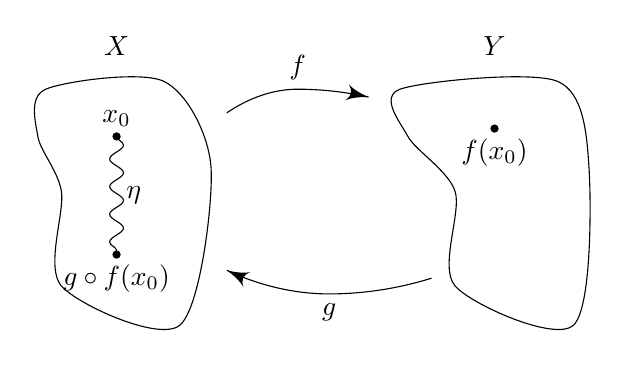
\begin{tikzpicture}
      \draw plot [smooth cycle] coordinates {(-3.7, -1.2) (-3.7, 0) (-4, 0.7) (-3.9, 1.3) (-2.4, 1.4) (-1.8, 0.3) (-2.2, -1.7)};
      \draw plot [smooth cycle] coordinates {(1.3, -1.2) (1.3, 0) (0.7, 0.7) (0.6, 1.3) (2.6, 1.4) (3, 0.3) (2.8, -1.7)};

      \node [circ] at (-3, 0.7) {};
      \node [above] at (-3, 0.7) {$x_0$};
      \node [above] at (-3, 1.6) {$X$};

      \node [above] at (1.8, 1.6) {$Y$};

      \node [circ] at (1.8, 0.8) {};
      \node [below] at (1.8, 0.8) {$f(x_0)$};

      \node [circ] at (-3, -0.8) {};
      \node [below] at (-3, -0.8) {$g\circ f(x_0)$};

      \draw [decoration={snake}, decorate] (-3, 0.7) -- (-3, -0.8) node [right, pos=0.5] {$\eta$};

      \draw [->] (-1.6, 1) parabola bend (-0.7, 1.3) (0.2, 1.2);
      \node [above] at (-0.7, 1.3) {$f$};

      \draw [->] (1, -1.1) parabola bend (-0.3, -1.3) (-1.6, -1);
      \node [below] at (-0.3, -1.3) {$g$};
    \end{tikzpicture}
  \end{center}
  We have no guarantee that $g\circ f(x_0) = x_0$, but we know that our homotopy $H'$ gives us $\eta = H'(x_0, \ph): x_0 \leadsto g\circ f(x_0)$.

  Applying our previous lemma with $\id_X$ for ``$f$'' and $g \circ f$ for ``$g$'', we get
  \[
    \eta_\# \circ (\id_X)_* = (g\circ f)_*
  \]
  Using the properties of the $_*$ operation, we get that
  \[
    g_*\circ f_* = \eta_\#.
  \]
  However, we know that $\eta_\#$ is an isomorphism. So $f_*$ is injective and $g_*$ is surjective.

  Doing it the other way round with $f\circ g$ instead of $g\circ f$, we know that $g_*$ is injective and $f_*$ is surjective. So both of them are isomorphisms.
\end{proof}


\begin{defi}[Simply connected space]
  A space $X$ is \textbf{simply connected} if it is path connected \textbf{and} $\pi_1(X, x_0) \cong 1$ for some (any) choice of $x_0 \in X$.
\end{defi}

\begin{eg}
  Clearly, a point $*$ is simply connected since there is only one path on $*$ (the constant path). Hence, any contractible space is simply connected since it is homotopic to $*$. For example, $\R^n$ is simply connected for all spaces.
\end{eg}



There is an important theorem, called the van Kampen theorem, for computations of fundamental groups. In the following, you will find the simple version of the theorem.
\begin{thm}[Simple version of van Kampen theorem]
If $X = U_1 \cup U_2$ with $U_i$ open and path-connected, and $U_1 \cap U_2$
path-connected and simply connected, then there is an isomorphism $\ \pi_1(U_1) * \pi_1(U_2) \cong \pi_1(X)$.
\end{thm}
Due to time limit, I have to omit general version of van Kampen theorem. 
If you are interested in it, you can read the book of Hatcher \cite[\S1.2]{Hatcher}.










\subsection{Covering space}

Intuitively, a \emph{covering space} of $X$ is a pair $(\tilde{X}, p: \tilde{X} \to X)$, such that if we take any $x_0 \in X$, there is some neighbourhood $U$ of $x$ such that the pre-image of the neighbourhood is ``many copies'' of $U$.
\begin{center}
  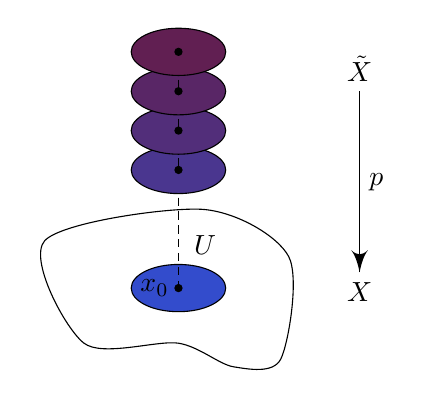
\begin{tikzpicture}
    \draw plot [smooth cycle] coordinates {(-1.2, -0.7) (0, -0.7) (0.7, -1) (1.3, -0.9) (1.4, 0.4) (0.3, 1) (-1.7, 0.6)};

    \draw [fill=mblue] ellipse (0.6 and 0.3);
    \node at (0.6, 0.3) [anchor = south east] {$U$};

    \draw [densely dashed] (0, 1.5) -- (0, 0);
    \foreach \y in {1.5, 2, 2.5, 3} {
      \node [circ] at (0, \y) {};
      \pgfmathsetmacro\c{100 - \y * 20};
      \draw [densely dashed] (0, \y) -- (0, \y - 0.5);
      \draw [fill=mblue!\c!mred] (0, \y) ellipse (0.6 and 0.3);
      \node [circ] at (0, \y) {};
    }
    \node [circ] at (0, 0) {};
    \node [left] at (0, 0) {$x_0$};

    \draw [->] (2.3, 2.5) node [above] {$\tilde{X}$}-- +(0, -2.3) node [pos=0.5, right] {$p$} node [below] {$X$};
  \end{tikzpicture}
\end{center}



\begin{eg}
  Consider $p_n: S^1 \to S^1$ (for any $n \in \Z\setminus\{0\}$) defined by $z \mapsto z^n$. We can consider this as ``winding'' the circle $n$ times, or as the following covering map:
  \begin{center}
    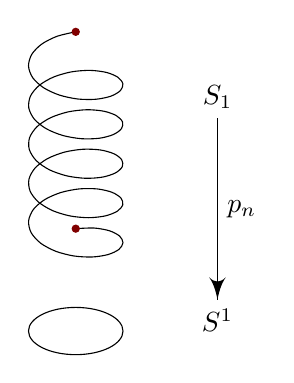
\begin{tikzpicture}
      \draw [samples=80, domain=0:5] plot [smooth] ({0.6 * sin (360 * \x)}, {1 + 0.3 * cos (360 * \x) + \x / 2});
      \node [circ, mred] at (0, 1.3) {};
      \node [circ, mred] at (0, 3.8) {};

      \draw ellipse (0.6 and 0.3);

      \draw [->] (1.8, 2.7) node [above] {$S_1$}-- +(0, -2.3) node [pos=0.5, right] {$p_n$} node [below] {$S^1$};
    \end{tikzpicture}
  \end{center}
  where we join the two red dots together.

  This time the pre-image of $1$ would be $n$ copies of $1$, instead of $\Z$ copies of $1$.
\end{eg}

\begin{eg}
  Consider $X = \RP^2$, which is the real projective plane. This is defined by $S^2/{\sim}$, where we identify every $x\simeq -x$, i.e.\ every pair of antipodal point. In fact, the quotient map $p: S^2 \to \RP^2$ is indeed a covering map, since the pre-image of a small neighbourhood of any $x_0$ is just two copies of the neighbourhood.  \begin{center}
    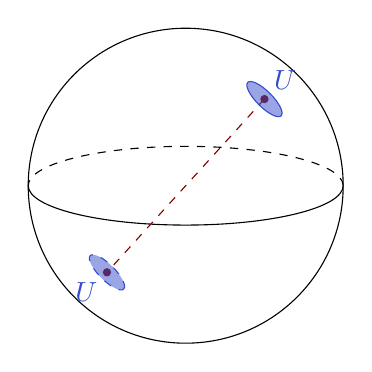
\begin{tikzpicture}
      \draw circle [radius=2];

      \draw [dashed] (2, 0) arc (0:180:2 and 0.5);
      \draw (-2, 0) arc (180:360:2 and 0.5);

      \draw [dashed, mred] (1, 1.1) node [circ] {} -- (-1, -1.1) node [circ] {};

      \draw [rotate around={-45:(1, 1.1)}, mblue, fill=mblue, fill opacity=0.5] (1, 1.1) ellipse (0.3 and 0.1) node [opacity=1, anchor = south west] {$U$};

      \draw [dashed, rotate around={-45:(-1, -1.1)}, mblue, fill=mblue, fill opacity=0.5] (-1, -1.1) ellipse (0.3 and 0.1) node [opacity=1, anchor = north east] {$U$};
    \end{tikzpicture}
  \end{center}

\end{eg}



\begin{defi}[Universal cover]
  A covering map $p: \tilde{X} \to X$ is a \textbf{universal cover} if $\tilde{X}$ is simply connected.
\end{defi}







\section{Homotopy group}

Let $I^n$ ($n\ge1$) denote the unitn-cube $I\times \cdots \times I$,
The boundary $\partial I^n$ is the geometrical boundary of $I^n$.
As in the fundamental group, we assume here that we shall be concerned with continuous maps $\alpha : I^n \to X$, which map the boundary $\partial I^n$ to a point $x_0 \in X$. Since the boundary is mapped to a single point $x_0$. The map $\alpha$ is called an $n$-loop at $x_0$. 

\begin{defi}[Homotopy class]
 Let $X$ be a topological space. The set of homotopy classes of $n$-loops ($n \ge 1$) at $x_0 \in X$ is denoted by $\pi_n(X, x_0)$ and called the $n$-th homotopy group at $x_0$. $\pi_n(X, x_0)$ is called the higher homotopy group if $n \ge 2$.
 \end{defi}
 
The product $\alpha * \beta$  just defined naturally induces a product of homotopy classes defined by
 $$[\alpha] * [\beta]=[\alpha * \beta] $$
\begin{figure}[h]\centering
\includegraphics[width=8cm]{homotopy-group}
\end{figure}



 Higher homotopy groups are always Abelian; for any $n$-loops $\alpha$ and $\beta$ at $x_0 \in X$, $[\alpha]$ and $[\beta]$  satisfy
$$[\alpha] * [\beta] = [\beta] * [\alpha].$$
 
 
\begin{figure}[h]\centering
\includegraphics[width=\textwidth]{homotopy-group2}
\end{figure}

\subsection{Global $SU(2)$ anomaly}
There are various applications of homotopy groups to physics. Here I just give you one example.

Let us consider the path integral of a gauge theory with chiral fermion $\psi$ in a representation $R$ of $G$.
\begin{equation}
Z[A_\mu] = \int [{\cal D} \psi][{\cal D}\bar\psi] e^{-\int \bar\psi D_\mu \sigma^\mu \psi}
\end{equation}  
To perform a further integration over $A_\mu$ consistently, we need \begin{equation}
Z[A_\mu]= Z[A^g_\mu], \quad A^g_\mu = g^{-1} A_\mu g  + g^{-1} \partial_\mu g.
\end{equation} for any gauge transformation $g:\mathbb{R}^4\to G$. We will learn it in a subsequent lecture about gauge transformation of non-Abelian gauge theory.


When we consider odd number of chiral fermions in the doublet of $\SU(2)$ gauge group, Witten has shown that there is a global anomaly \cite{Witten:1982fp}.
Since continuous change of $g$ does not change the phase of $[{\cal D}\psi][{\cal D}\bar \psi]$, we need to consider maps $g:\mathbb{R}^4\to \SU(2)$ up to continuous change. Upon one-point compactifiction of $\bR^4$ to $S^4$,
they are characterized by $\pi_4(\SU(2))$, which is known  
\begin{equation}
\pi_4(\SU(2))=\pi_4(S^3)=\mathbb{Z}_2~.
\end{equation} Let $g_0:\mathbb{R}^4\to \SU(2)$ be the gauge transformation corresponding to the nontrivial element in this $\bZ_2$.  
It is known that  $[{\cal D}\psi][{\cal D}\bar \psi]$ gets a minus sign  under this gauge transformation.
So, one cannot have an odd number of Weyl fermions in the doublet representation of gauge group $\SU(2)$. 



\begin{thebibliography}{99}
\bibitem{Witten:1982fp}
E.~Witten, {\it An SU(2) Anomaly}, Phys.Lett. \textbf{B117} (1982) 324-328


\bibitem{Hatcher}
A.~Hatcher, {\it Algebraic Topology}, \url{https://www.math.cornell.edu/~hatcher/AT/AT.pdf}
\end{thebibliography}

\end{document}
